\documentclass{article} 
\usepackage[]{authblk}

\usepackage{pslatex} \usepackage{apacite} \usepackage {graphicx} 
\usepackage [sort]{natbib} 
\usepackage{qtree} 
\usepackage[margin=10pt,labelfont=bf]{caption} 
\usepackage{fancyhdr}
\usepackage[nottoc]{tocbibind} %\usepackage[perpage]{footmisc} \usepackage{paralist}
\usepackage{amsmath,amsthm,amssymb} 
\usepackage{tipa} \usepackage{amsmath,amsthm,amssymb} 
\usepackage{tipa}
\usepackage{csvtools} 
\usepackage[T1]{fontenc} 
\usepackage{datatool} %\usepackage{glossaries}
\usepackage[]{float} 
\usepackage{hyperref} 
\usepackage[]{placeins} 

\title{Clustering in efficient lexical
design}

%%%analysis comes from lexicon/analysis folder lex_analysis.R
%%%lexicon/wiki/analysis.R


\begin{document}

\maketitle



\textbf{Keywords:} linguistics, lexical design, communication, phonotactics,

\begin{abstract}
\end{abstract}


\section{Introduction} Saussure famously stated that there is an arbitrary relationship between word forms and
their meanings. As \cite{hockett1960origin} wrote, ``The word `salt' is not salty nor granular; `dog' is not
`canine'; `whale' is a small word for a large object; `microorganism' is the reverse.'' Our ability to
manipulate such arbitrary symbolic representations is one of the hallmarks of human language and, in fact,
makes language richly communicative since it permits reference to arbitrary entities, not just those that have
iconic representations \citep{hockett1960origin}.\footnote{\cite{monaghan_arbitrariness_2011} and
\cite{Gasser2004origins} note that arbitrariness may also be a boon to learning in that, if there were a tight
relationship between form and meaning, semantically similar entities like \textit{dog} and \textit{cat} would
have similar names (perhaps \textit{dog} and \textit{tog}). Such a system would increase the chance of
perceptual confusability since those words are often used in similar contexts and so context alone would not
always be able to disambiguate the words.}

Exceptions to the arbitrariness of linguistic symbols are few and, in some sense, prove the rule. For
instance, there is a tendency in English for \textit{gl-} words to be associated with light reflectance as in
``glimmer,'' ``gleam,'' and ``glisten'' \citep{bergen_psychological_2004}. There are additionally
cross-linguistic correspondences between form and meaning, such as a tendency for words referring to smallness
to contain high vowels \citep{hinton2006sound,sapir1929study}. More broadly, it has been shown that speakers
can distinguish between different classes of words, such as concrete versus abstract nouns, based on phonetic
properties \citep{reilly_arbitrary_2012}. These examples are notable not for their regularity, but for their
rarity and lack of systematicity. Even representations of animal noises, for instance, differ across languages
(compare English ``cockadoodledoo'' to Spanish ``cocorico''). Languages' choice of non-onomatopoeic words is
even more the result of historical accident: there is no systematic reason why we call a dog a \textit{dog}
and a cat a \textit{cat} instead of the other way around, or instead of \textit{chien} and \textit{chat}. As a
result of this widespread arbitrariness, there are many degrees of freedom in how a lexicon is structured.
Lexicons can vary in their distribution of word lengths, in their distribution of phonemes, in how they carve
out the semantic space, what wordforms they choose, and in many other properties.

The existence of an information storage and processing system that allows such a high degree of freedom and
arbitrariness is unusual in human cognition. The way in which languages use this freedom is potentially
informative about the underlying forces shaping human communication and thought. Specifically, we might expect
that over time our capacity for arbitrary word meanings has led to an essentially random or non-systematic
distribution of wordforms--at least among monomorphemic words, which are the focus of this
study.\footnote{There is, of course, an obvious source of regularity in morphologically complex words like
``happiness,'' in which the words are formed from regular parts.} This landscape of randomly distributed
wordforms is the default hypothesis a pure Saussurean might make. On the other hand, it is easy to imagine
that in the face of minimal constraints beyond phonotactics on the set of well-formed words a language may
use, lexicons might evolve under other pressures---perhaps for communicative or cognitive optimization.

In fact, communicative and cognitive optimization may yield very different types of lexicons. If we assume a
noisy channel model of communication \citep{shannon_mathematical_2001,
levy_expectation-based_2008,gibson2013noisy}, there is always some chance that the linguistic signal will be
corrupted through errors in production, errors in comprehension, or some other form of noise in the signal. A
lexicon is maximally robust to noise when the expected phonetic distance between words is maximized
\citep{flemming_contrast_2004, graff_2012}, an idea used in error-correcting codes
\citep{shannon1948mathematical}. Such sparsity has been observed in phonetic inventories
\citep{hockett1955manual,flemming2002auditory} in a way that is sensitive to phonetic context
\citep{steriade1997phonetics,steriade2001directional}. Applying this idea to the set of wordforms chosen in a
lexicon, one would expect wordforms to be maximally dissimilar from each other, given the bounds of
phonotactics and conciseness.

The pressure for dispersion becomes apparent when one considers that it seems almost absurd to imagine a
language that has many long words that sound almost identical to other long words. While English has words
like `accordion' and `encyclopedia,' it certainly does not also have `accordiom' or 'encyclofedia.' Such
forces may influence coining and borrowing; it seems plausible, for instance, that the 16th-century French
borrowing `caparison' (a type of horse covering) has remained very infrequent in English because it is
extremely likely to be misheard as the far more frequent `comparison.'

Another force, however, conflicts with the pressure for sparsity in the lexicon: there is a pressure for the
lexicon to be easy to learn, remember, produce, and process. In the most extreme possible case, one might
imagine a language with only one wordform. Learning the entire lexicon would, in this case, be as simple as
learning to remember and pronounce one word. While this example is extreme effects of systematicity and re-use
can be found at every level of the lexcion. There are complex constraints that govern the set of sounds
allowed in any given language \citep{hayes_blick_2012}. Words can be regularly formed and stored using
prefixes and suffixes \citep{odonnell_productivity_2011}. \cite{monaghan_arbitrariness_2011} show that this
phonetic regularity helps language learners group words into categories. \cite{storkel_differentiating_2006}
show that adult learners more easily learn non-words that appear in high-density phonological neighborhoods,
where a phonological neighbor is defined as a word that differs from the target word by just one sound. These
results are unsurprising since human memory is known to improve when information can be shared across
different modalities.

The pressure for re-use manifests itself quite clearly in domains like phonology and morphology. While there
are many possible sounds sequences that can exist in human languages, any given language relies on a
relatively small subset of those sounds. And, by having regular suffixes like \textit{ness} and \textit{esque}
that can derive new forms, it becomes possible to understand novel words through decomposition. It is this
regularity that allows us to understand a word like \textit{Twitter-esque}, even if we have never seen it
before.

The basic challenge with assessing these forces---and comparing them to a truly arbitrary or non-systematic
lexicon----is that it is difficult to know what standard existing lexicons should be compared to. If we
believe, for instance, that the wordforms chosen by English are sparse, we must be able to quantify sparseness
\emph{compared to} some baseline. Here, we present a novel method for solving this methodological puzzle, and
we use it to study the fundamental forces shaping the set of monomorphemes chosen by the English
lexicon\footnote{Prior theoretical arguments about the statistics of language---in particular Zipf's law
\cite{mandelbrot_informational,miller1957some}---have made use of a \emph{random typing} model in which
sub-linguistic units are generated at random, occasionally leading to a word boundary when a ``space''
character is emitted. This model makes extremely unrealistic assumptions about the true generative processes
of language \cite{howes1968zipf,piantadosi2012information} and therefore provides a poor baseline for studying
the true statistical forces of human languages.}.


\section{Neighborhood and frequency effects} 

As a first pass at evaluating the extent to which languages show a preference for re-use, we investigated
whether (a) words that are orthographically likely are more likely to be frequent than words that are less
orthographically probable and (b) whether words in dense neighborhoods are more likely to be frequent than
words with few neighbors.

\subsection{Method} We used a corpus of 115 languages downloaded from Wikipedia and restricted our analysis to
the top 20,000 most frequent wordforms in each language. We used exclusively orthographic wordforms here,
which we believe are a reasonable proxy for phonetic forms. One natural test statistic is \emph{phonological neighborhood density} (PND),
which focuses on 1-edit pairs. PND is defined for each word as the number of other words in the lexicon that
are one edit (an insertion, deletion, or substitution) away in phonetic space
\citep{luce1986neighborhoods,luce1998recognizing}. For instance, `cat' and `bat' are phonological neighbors,
as well as minimal pairs since they have the same number of letters and differ by 1. `Cat' and `cast' are
neighbors but not minimal pairs.
Neighborhood density has been shown to affect a wide variety of lexical processing from reaction time
\citep{vitevitch1998words} to fMRI activation of language areas \citep{prabhakaran2006event}.

For each word in each language, we computed the
number of minimal pairs and neighbors that the word had among the 20,000 wordforms in the sample. We also
trained a 3-phone model (smoothed and with backoff) on each set of 20,000 words and used the language model to
find the probability of each word string under the model. EXAMPLE OF HIGH AND LOW.

\subsection{Results} 


Figures \ref{probvfreq} and \ref{neighborsvfreq} show density plots of scaled orthographic probability versus
scaled log frequency and scaled number of neighbors versus scaled frequency, respectively, for 4-letter words.
The positive slope of the red line reveals a correlation, in almost all languages, between these variables.


\begin{figure}[htbp]
  \centering
  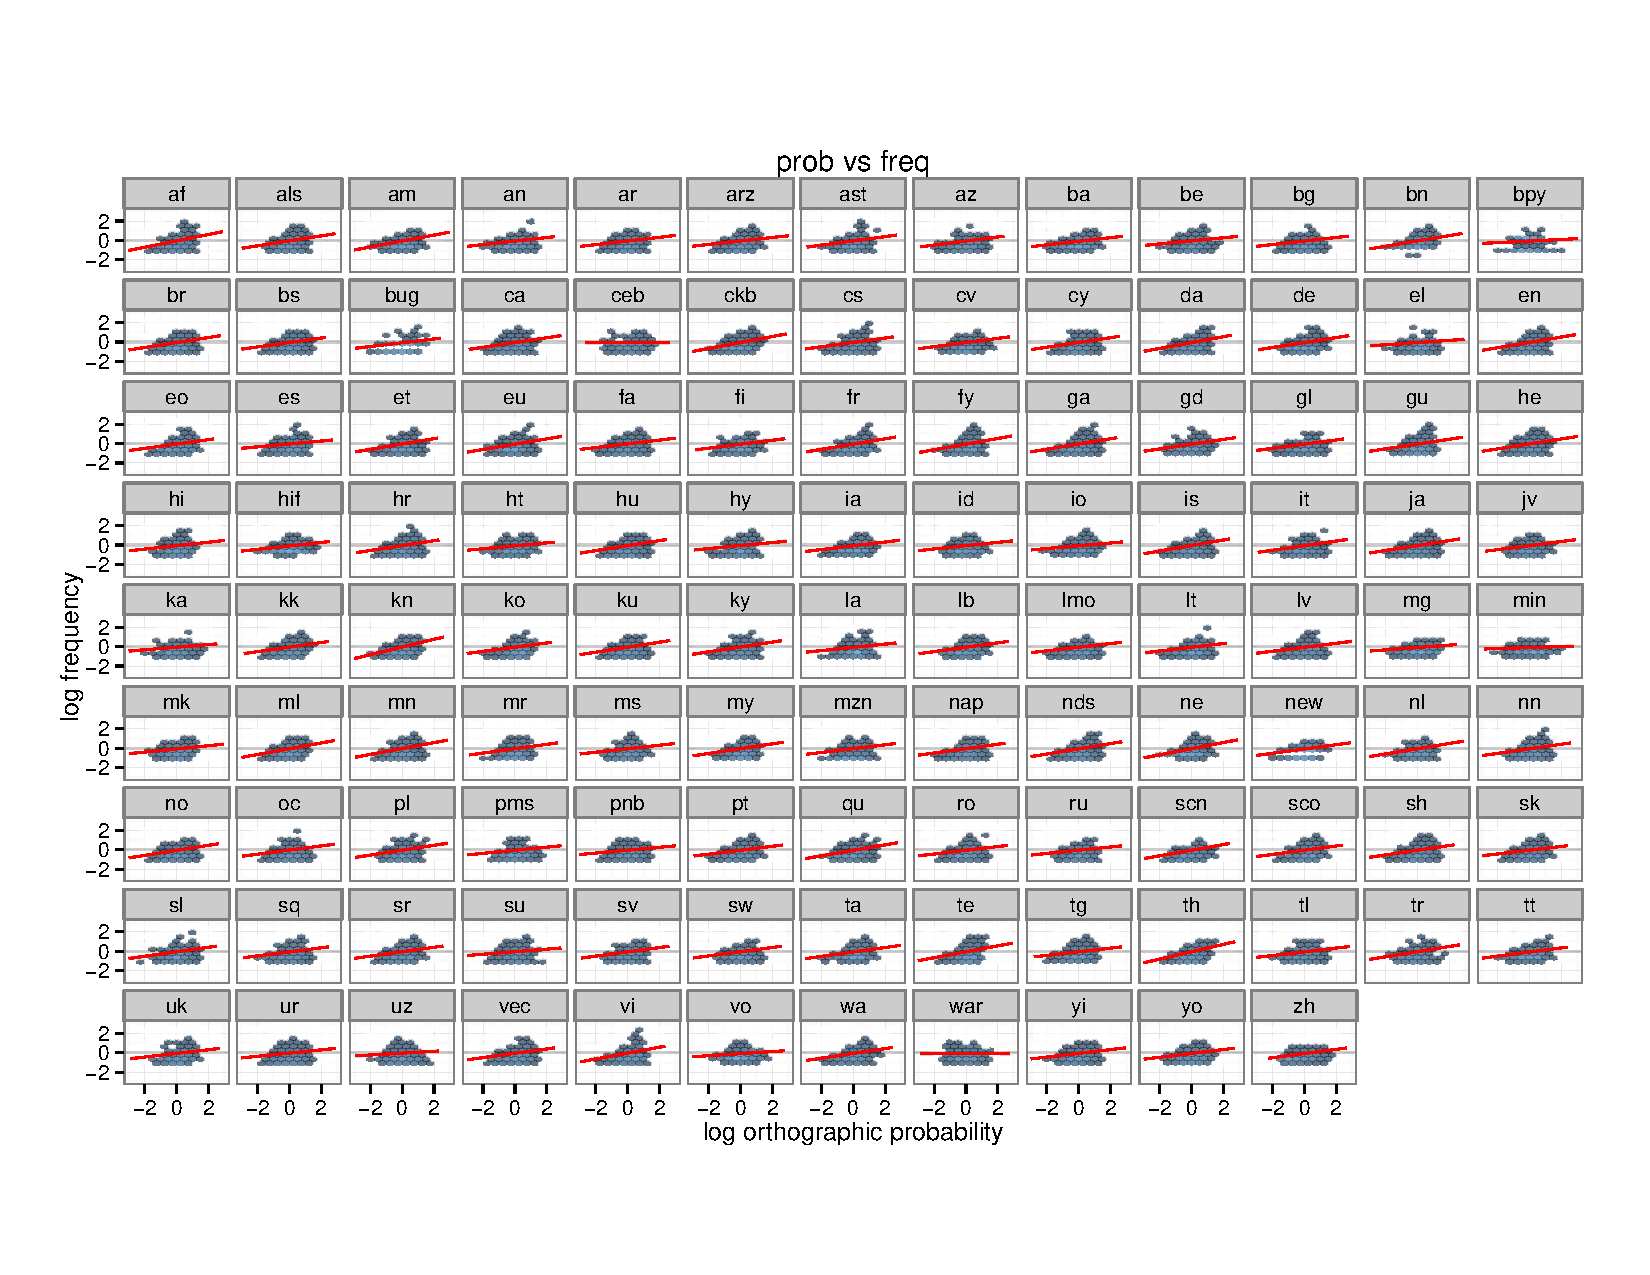
\includegraphics[width=0.8\textwidth]{PDFs/big_cor2_probvfreq.pdf}
  \caption{Orthographic probability plotted against frequency. The red line is a line of best fit.}
  \label{probvfreq}
\end{figure}

\begin{figure}[htbp]
  \centering
  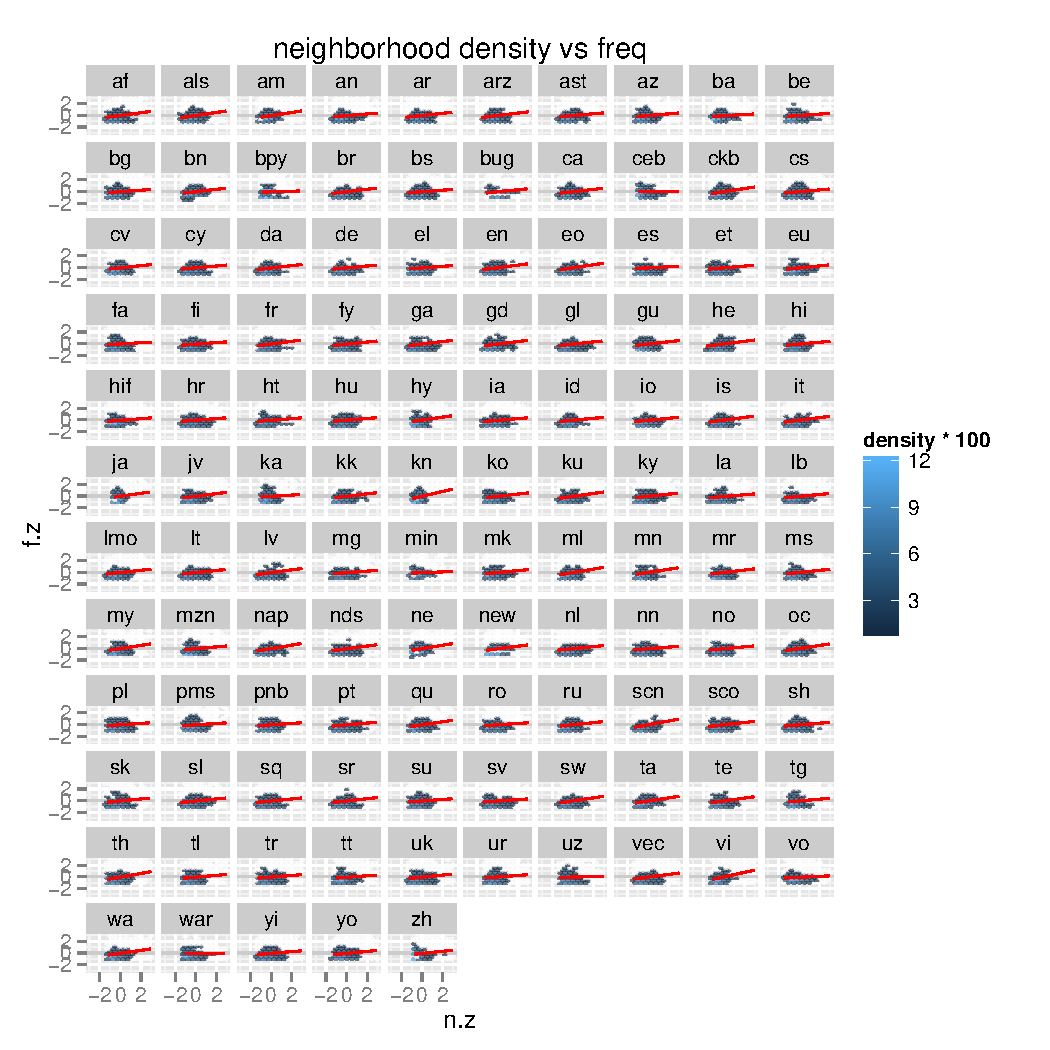
\includegraphics[width=0.8\textwidth]{PDFs/big_cor2_neighborsvsfreq.pdf}
  \caption{Number of orthographic neighbors plotted against frequency. The red line is a line of best fit.}
  \label{neighborsvfreq}
\end{figure}

Using Spearman correlations to obtain non-parametric correlation coefficients, analyzing
each length separately, we found
that almost all languages show significant correlations between log frequency and orthographic probability
(mean r = .22 averaging across the individual correlation for each length and language),
between log frequency and number of neighbors (mean r = .22), between log frequency and number of minimal
pairs (mean r = .18), and
(unsurprisingly) between orthographic probability and number of minimal pairs (mean r = .50) and between orthographic
probability and number of neighbors (mean r = .54). Figure \ref{cor.test} shows this graphically by length.

\begin{figure}[htbp]
  \centering
  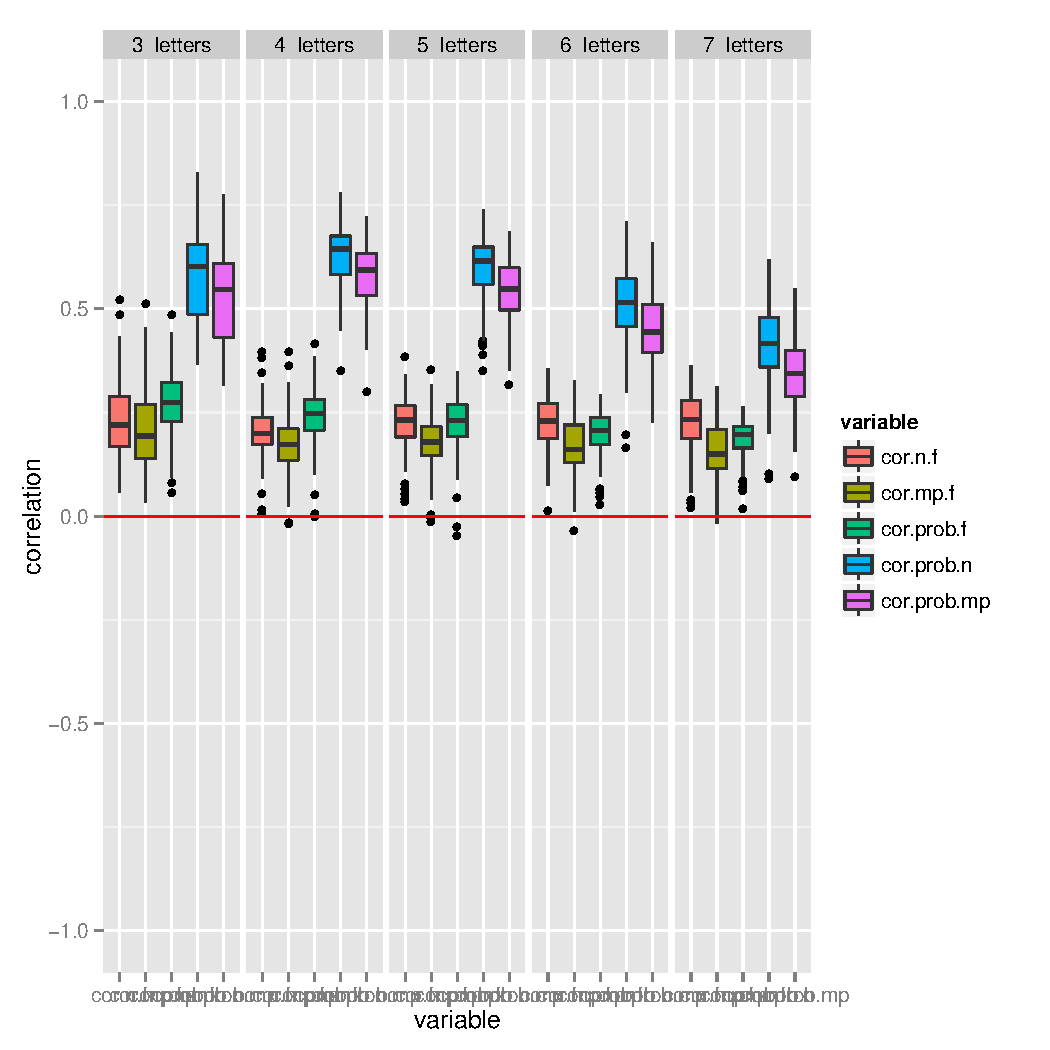
\includegraphics[width=0.8\textwidth]{PDFs/violins_of_stats.pdf}
  \caption{Each bar shows the mean correlation across languages for the variable shown. ``n'' here refers to
    number of neighbors, ``f'' is log frequency, ``mp'' is minimal pairs, and ``prob'' is orthographic
    probability as measured by the 3-phone model.}
  \label{cor.test}
\end{figure}


Table \ref{cor.table} shows the number of correlations for each variable, for each length, that are not
significant out of 115. For each contrast, the vast majority of languages show a significant correlation in
the expected direction.

\begin{table}[ht]
\centering
\begin{tabular}{rlrrrrr}
  \hline
 & variable & 3  letters & 4  letters & 5  letters & 6  letters & 7  letters \\ 
  \hline
1 & cor.mp.f.p &   5 &   4 &   4 &   6 &  11 \\ 
  2 & cor.n.f.p &   3 &   3 &   2 &   2 &   4 \\ 
  3 & cor.prob.f.p &   3 &   3 &   3 &   2 &   2 \\ 
  4 & cor.prob.mp.p &   0 &   0 &   0 &   0 &   1 \\ 
  5 & cor.prob.n.p &   0 &   0 &   0 &   0 &   0 \\ 
   \hline
\label{cor.table}
\end{tabular}
\end{table}


\subsection{Discussion}

Unsurprisingly, we found a robust correlation between orthographic probability and number of neighbors/minimal
pairs. This result holds for all lengths across the vast majority of languages and is consistent with what we
should expect. The word ``set'' is more likely to have neighbors in English than the word ``quiz'' simply
because the letters in ``set'' are more common. So, probabilistically, there are more opportunities for a word
to be orthographically close to ``set'' than to ``quiz.''

Perhaps more interesting is the correlation between neighborhood density and frequency and between orthographic
probability and frequency. A prior, it is not obvious that we should see this effect since frequency is not
used in computing orthographic probability. The result suggests that, if a word has many neighbors and/or has
high orthographic probability, it is
more likely to be frequent. 

One explanation for this relationship between frequency and orthographic probability is apparent when we
imagine words being probabilistically generated by an orthographic model. That is, when we need a meaning for
a new word, we generate a wordfrom from our 3-phone model. Words that are more likely will be independently generated more
often, which would allow their frequency to increase. Consider homophones like ``pore'', ``pour'', and
``poor'.'' These words have no recent shared etymological ancestry but all ended up with the same phonetic
pronunciation in English because the phonetic string is quite likely. Therefore, the frequency of the sound
string is inflated by corresponding to multiple meanings. Thus, the phonetic probability could give rise to
higher frequency for the string. And, of course, we already have seen that higher string probability gives
rise to more neighbors.

In the next section, we present results from an experiment that compares the natural language lexicon to a
plausible baseline.

CITE OLD RESULTS. BAAYEN?

\section{Null lexicon experiments}

\subsection{Lexicons} Because we want to evaluate the real lexicons of mono-morphemic words relative to
baselines, we focus on languages for which we could obtain reliably marked morphological categories. For
English, German, and Dutch, we use CELEX pronunciations and restrict the lexicon to mono-morphemic words
(words marked M). For French, we used Lexique, and I.D. (a native French speaker) identified mono-morphemic
words by hand. For simplicity, we study as the `real lexicon' a subset of the English lexicon consisting of
all words of 4 to 8 phones\footnote{Three-phone words were excluded because they tend to have a phonotactics
distinct from longer words (typically only CVC), and longer words were excluded because any two words of 9
letters or more are unlikely to have very much overlap, so it becomes difficult to compare.} from the CMU
corpus \citep{weide1998cmu}, as modified for the BLICK phonotactic probability calculator using the default
English grammar with stress \citep{hayes_blick_2012}.

In order to avoid the effect of homophones, we allowed only unique pronunciations. We define the lexicon to be
the set of unique pronunciations in CELEX.

All three CELEX dictionaries were transformed to make diphthongs into 2-character strings. From the English
CELEX, we removed a small set of words containing foreign characters. The lexicons used for each language are
included in Appendix A.
 
\subsection{Choosing the best null model}

\subsubsection{Method} In order to evaluate the real lexicon against a plausible baseline, we first defined a
number of baseline lexical models, which we describe below:

\begin{itemize}

\item n-phone models: For n from 1 to 5, we trained a language model over n phones. Like an n-gram model over
words, the n-phone model lets us calculate the probability of generating a given letter after having just seen
the previous {\it n-1} letters: $P(x_i | x_{i - (n-1)},...,x_{i-1})$. To avoid overfitting the model, we used
backoff and smoothing. The smoothing parameter was set by doing a sweep over possible parameters and choosing
the one that maximized the probability of the held-out set.

\item n-syll models: For n from 1 to 2, we trained a language model over syllables. This generative procedure
is like the n-phone model, but we instead train over syllables.

\item PCFG: **ISABELLE**

\end{itemize}

In order to evaluate their ability of each model to capture the structure of the real lexicon, we trained each
model on 75\% of the lexicon and evaluated the probability of generating the remaining 25\% of the lexicon.

\subsubsection{Results} The parameter sweep revealed that the optimal smoothing parameter was .01. In all
models described, unless otherwise stated, we use .01 as the smoothing parameter.

As shown in , the 5-phone model is the best performer across all languages.

PUT FIGURE HERE


\subsection{Results}

We simulated 30 lexicons of each type and computed test statistics for the real lexicon and each of the
simulated lexicons. As described above, we then compared the distribution of this statistic across the
simulated lexicons to its value in the real lexicon and compared the real lexicon to each of the null models.
Below, we describe these measures and use them to characterize how the simulated lexicons from the generative
model compare to the real lexicon of each language that we tested.


 
To compare lexicons, it is necessary to define a number of test statistics that can be computed on each
lexicon to assess how it uses its phonetic space. Just like in classic null hypothesis testing, we compute a
z-score using the mean and standard deviation estimated from the 50 lexicons generated by our ``null'' lexicon
model. We then ask whether the real lexicon value falls outside the range of values that could be expected by
chance under the null model. The p-value in the tables reflects the probability that the real lexicon value
could have arisen by chance under the most tightly constrained generative model.

\subsubsection{Minimal pairs} 

\begin{figure} \centering
  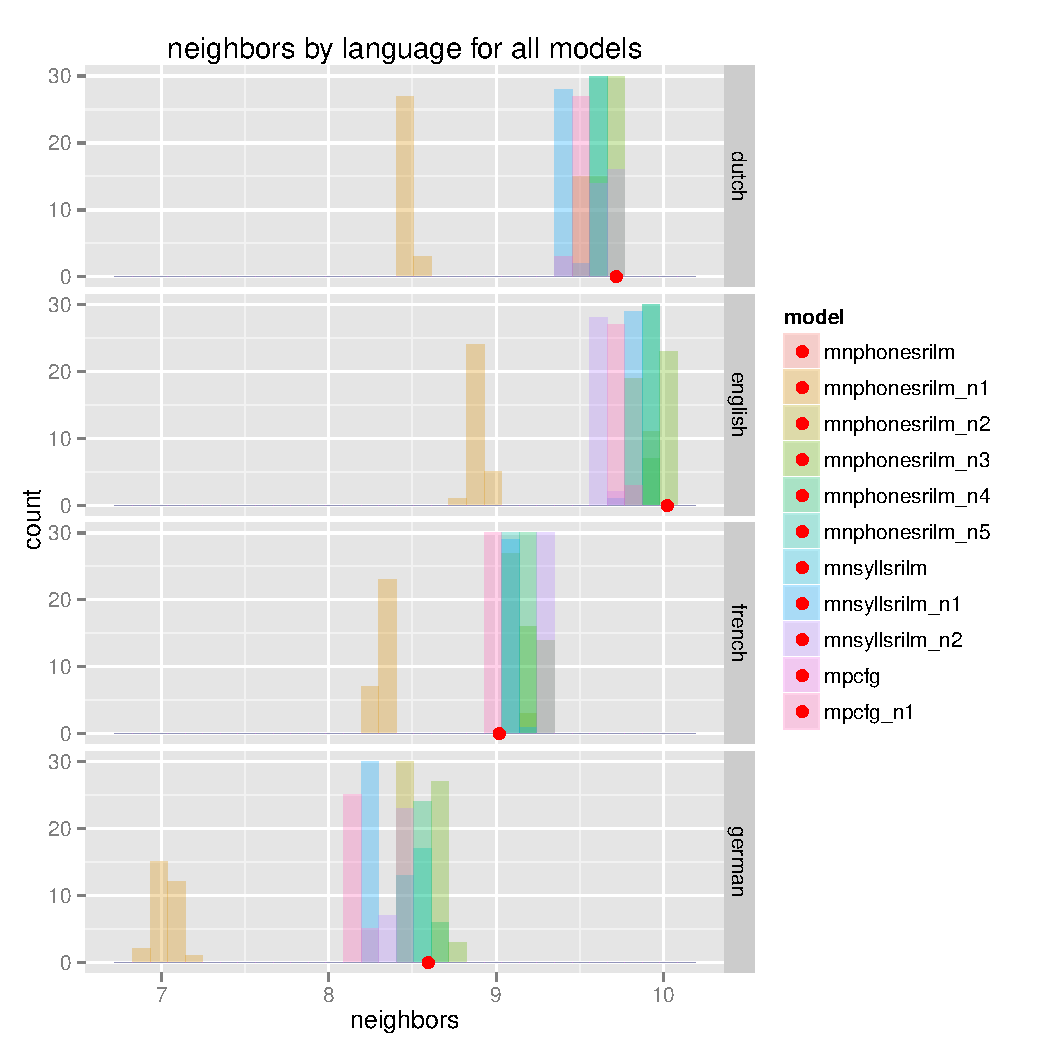
\includegraphics[width=0.8\textwidth]{PDFs/neighbors_all_models.pdf}
  \caption{Each colored histogram represents a distribution of minimal pair counts, broken up by word length
in phonemes, across the 50 simulated lexicons from each of the four generative models. The y-axis shows the
log number of minimal pairs per 10,000 words for each of the four types of lexicons. The red dot shows the
real lexicon value for each condition. The most tightly constrained generative model (CV and phonotactically
matched) comes closest to matching the real lexicon value in all cases, but all of the histograms for all of
the lengths fall to the left of the red dot, which suggests that the real lexicon has more minimal pairs than
any of the simulated ones.}
  \label{fig:pairs}
\end{figure}



Figure \ref{fig:pairs} summarize these hypothesis tests, showing how the various simulated lexicons compare to
the real lexicon in terms of log number of minimal pairs per 10,000 words for words of varying length. For
words of 6 phones and above, minimal pairs are quite rare, but the same pattern holds. Each color represents a
different type of generative model. The red
dot represents the real lexicon value.

Because not all sounds are equally confusable (`p' and `b' are far more confusable than `p' and `e'; see
\cite{graff_2012} ), we also look specifically at phonological neighbors whose minimal difference relies on a
subtle contrast between a voiced and unvoiced consonant. To check whether the clumpiness effect holds even for
minimal pairs that are phonetically confusable (i.e., minimal pairs that differ only by a voicing contrast as
in pig/big and mad/mat), we additionally compared the real lexicon and the simulated ones in terms of minimal
pairs that differ only in phonetically similar stop consonants: `p/b', `t/d', and `k/g'. The real lexicon has
more such minimal pairs than even the most constrained generative model. minimal pairs from the most tightly
constrained generative model (length, CV, and phonotactically matched). The red dot represents the real
lexicon value, and the dotted lines represent 95\% confidence intervals based on the simulated values. In all
cases, the red dot falls well to the right of the dotted line, indicating that the real lexicon has
significantly more of each type of minimal pair.


\begin{figure}
\centering 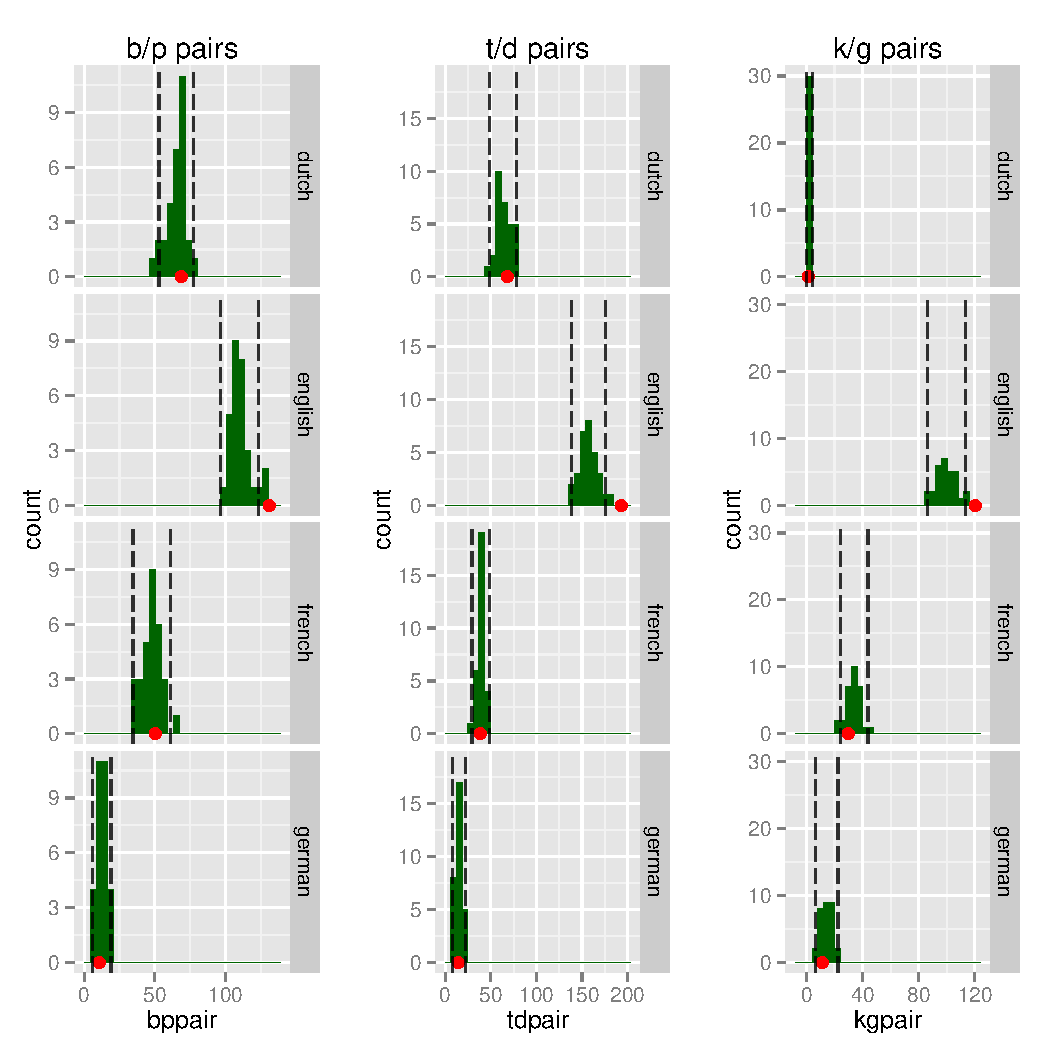
\includegraphics[width=0.8\textwidth]{PDFs/specific_mps.pdf}
  \caption{These histograms show the distribution of the most closely matched simulated lexicon (in green)
compared to the real lexicon (the red dot) in terms of confusable minimal pairs: `p/b', `k/g', and `t/d'. The
dotted lines represent 95\% confidence intervals derived from the distribution of simulated lexicons. In all
cases, the red dot is significantly to the right of the simulated lexicon distribution--which suggests that
the real lexicon is clumpier than expected by chance. }
  \label{3pairs}
\end{figure}

\subsubsection{Word onset measures} Besides phonological neighbors, there is evidence that word onsets are of
particular importance in lexical processing \citep{marslen1980speech,marslen1987functional,wingfield1997word},
so we also compute several test statistics that focus on shared word onsets. For instance, we looked at the
percent of the lexicon that could be disambiguated after seeing only $n$ sounds.

To see whether word onsets show clustering in the real lexicon, we looked at the percent of words in the real
lexicon that are able to be uniquely disambiguated after 3 sounds and 4 sounds. The words {\em cap} and {\em
cat}, for instance, can be disambiguated from each other after 3 sounds, but not Figure \ref{3onset} shows
histograms for each of these measures. The red dot representing the real lexicon shows that the real lexicon
has significantly more confusable onsets than the simulated lexicons.


\begin{figure}
\centering 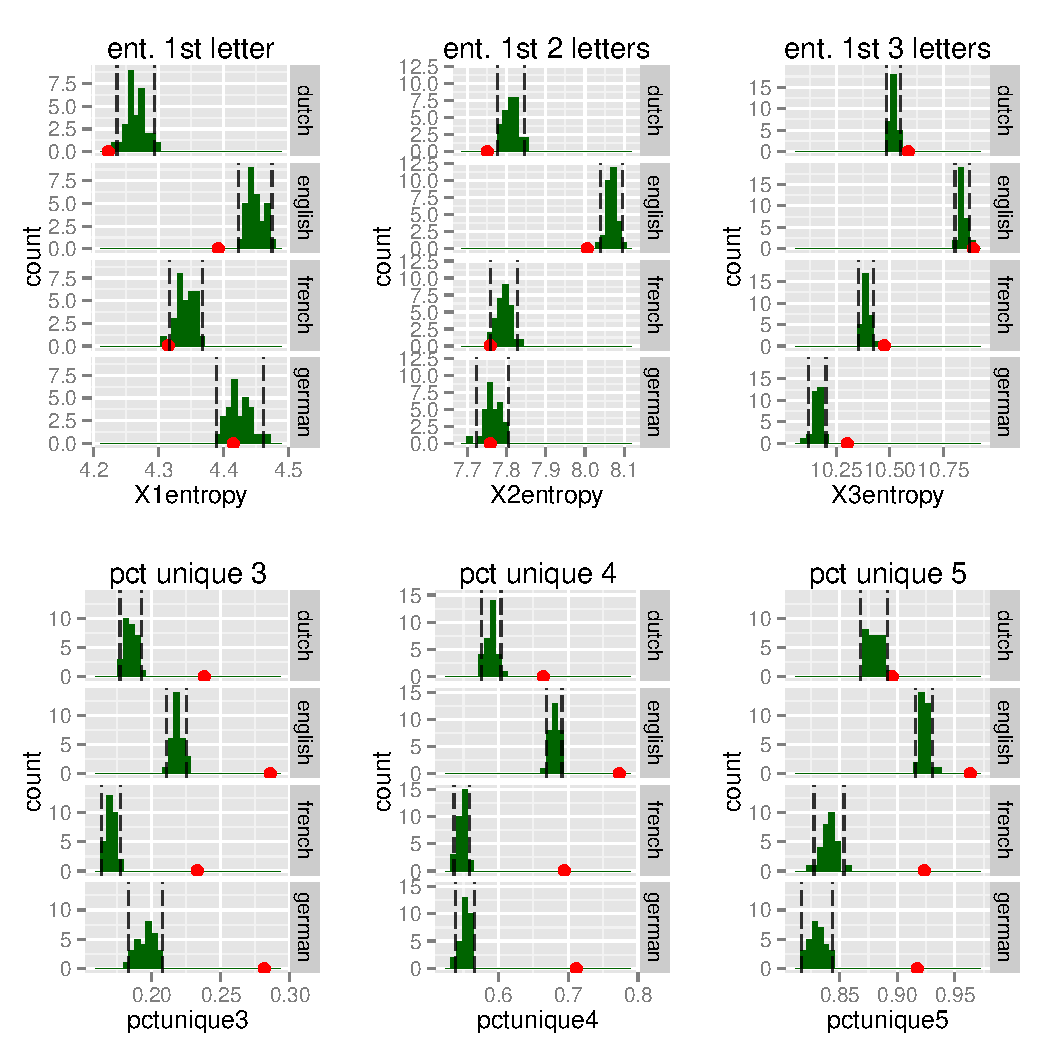
\includegraphics[width=0.8\textwidth]{PDFs/onset_n5.pdf}
  \caption{NEED }
  \label{3onset}
\end{figure}

\subsubsection{Levenshtein distance}

We can evaluate clustering using more global measures by considering the average string edit distance
(\textit{Levenshtein distance}) between words. The Levenshtein distance between two sound strings is simply
the number of edits required to get from one string to another.\footnote{So, the Levenshtein distance between
`cat' and `cast' is 1 (insert an `s'), and it is 2 between `cat' and `bag' (c $\rightarrow$ b, t $\rightarrow$
g). A possible objection to using Levenshtein distances is that there is little apparent difference in
phonological confusability between a pair like `cats' and `bird', which has a Levenshtein distance of 4, and a
pair like `cats' and `pita,' which has a Levenshtein distance of only 3 but which is arguably even more
different since it differs in syllable structure. Ultimately, neither pair is especially confusable: the
effects of phonological confusability tail off after 1 or 2 edits. }.

In the remainder of the results, we will focus mainly on the most tightly generative model (CV and
phonotactically matched)


\begin{figure} \centering
  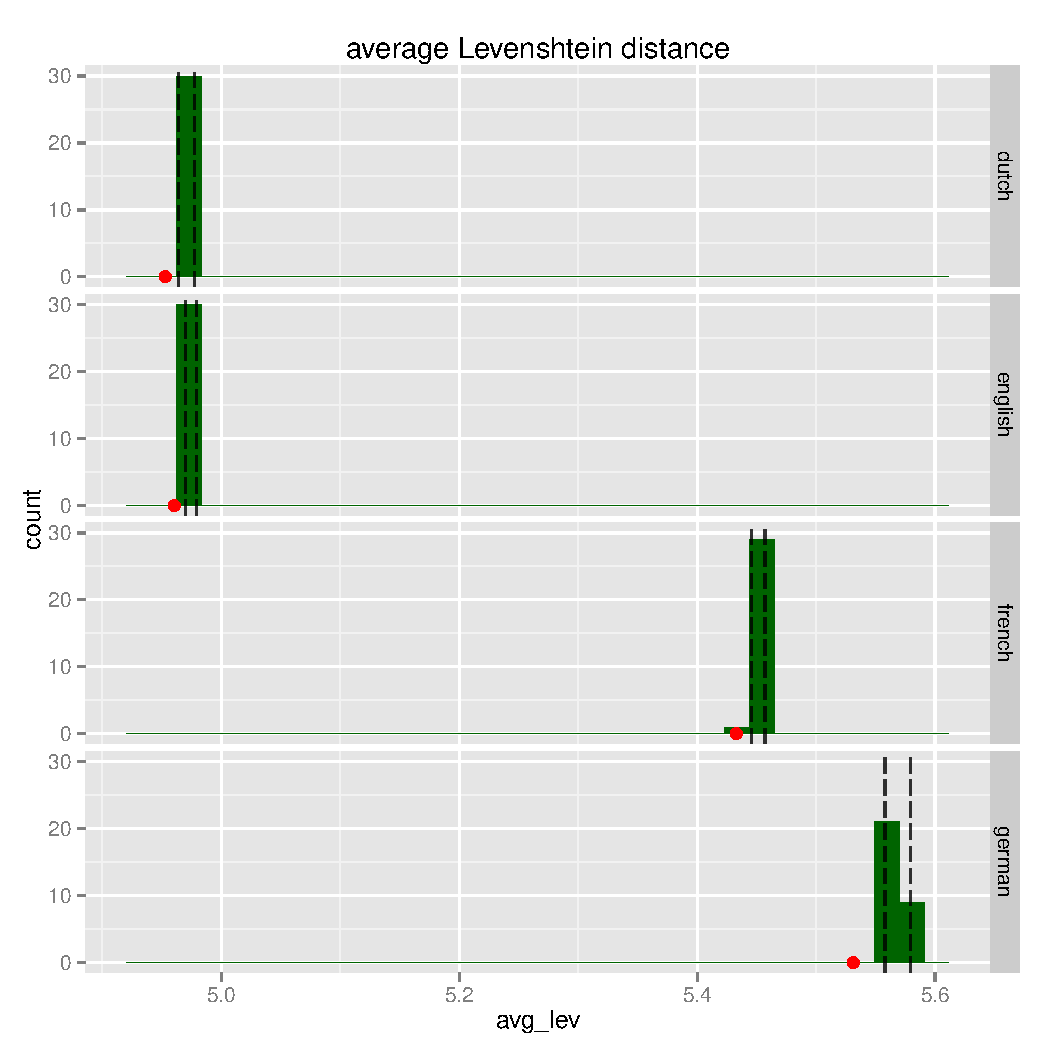
\includegraphics[width=.8\textwidth]{PDFs/avg_lev_n5.pdf}
  \caption{The histograms show the distribution of average Levenshtein distances for each of the 50 simulated
lexicons (restricted to only the most closely matched generative model). The red dot represents the real
lexicon's value, and the dotted lines are 95\% confidence intervals.}
  \label{levs}
\end{figure}



\subsubsection{Network measures}

Simply calculating phonological neighbors and onset confusability, however, does not tell us everything about
how sounds are distributed across a lexicon. Do certain words have many neighbors and others very few? Or do
neighbor pairs tend to be more uniformly distributed across the lexicon? To answer these questions, we
construct a phonological neighborhood network as in \cite{arbesman_structure_2010}, whereby we build a graph
in which each word is a node and any phonological neighbors are connected by an edge, as in the toy example in
Figure \ref{fig:toy}.

Using techniques from network analysis that have been fruitfully applied to describe social networks and other
complex systems \citep{wasserman1994social,watts1998collective,barabasi1999emergence}, we can better
characterize the clustering behavior of the lexicon. We use measures like \emph{average clustering
coefficient}, \emph{transitivity}, and percent of nodes in the \textit{giant component} to evaluate how
tightly clustered nodes in a network are. A graph's transitivity is the ratio of the number of triangles (a
set of 3 nodes in which each node in the set is connected to both other nodes in the set) to the number of
triads (a set of 3 nodes in which at least two of the nodes are connected). Thus, transitivity in effect asks,
given A is connected to B and B is connected to C, how likely is it that A is also connected to C? The average
clustering coefficient is a closely related measure that find the average clustering coefficient across all
nodes, where the clustering coefficient of a node is defined as the fraction of possible triangles that
\textit{could} go through that node that actually do go through that node. Both of these measure the extent to
which nodes cluster together. The largest cluster in a network is known as the giant component. A network with
many isolated nodes will have a relatively small giant component, whereas one in which nodes are tightly
clustered will have a large giant component. Applying these measures to the lexicon gives insight into lexical
structure not captured by just the number of neighbors or by Levenshtein distance.

\begin{figure}[htbp] \centering
 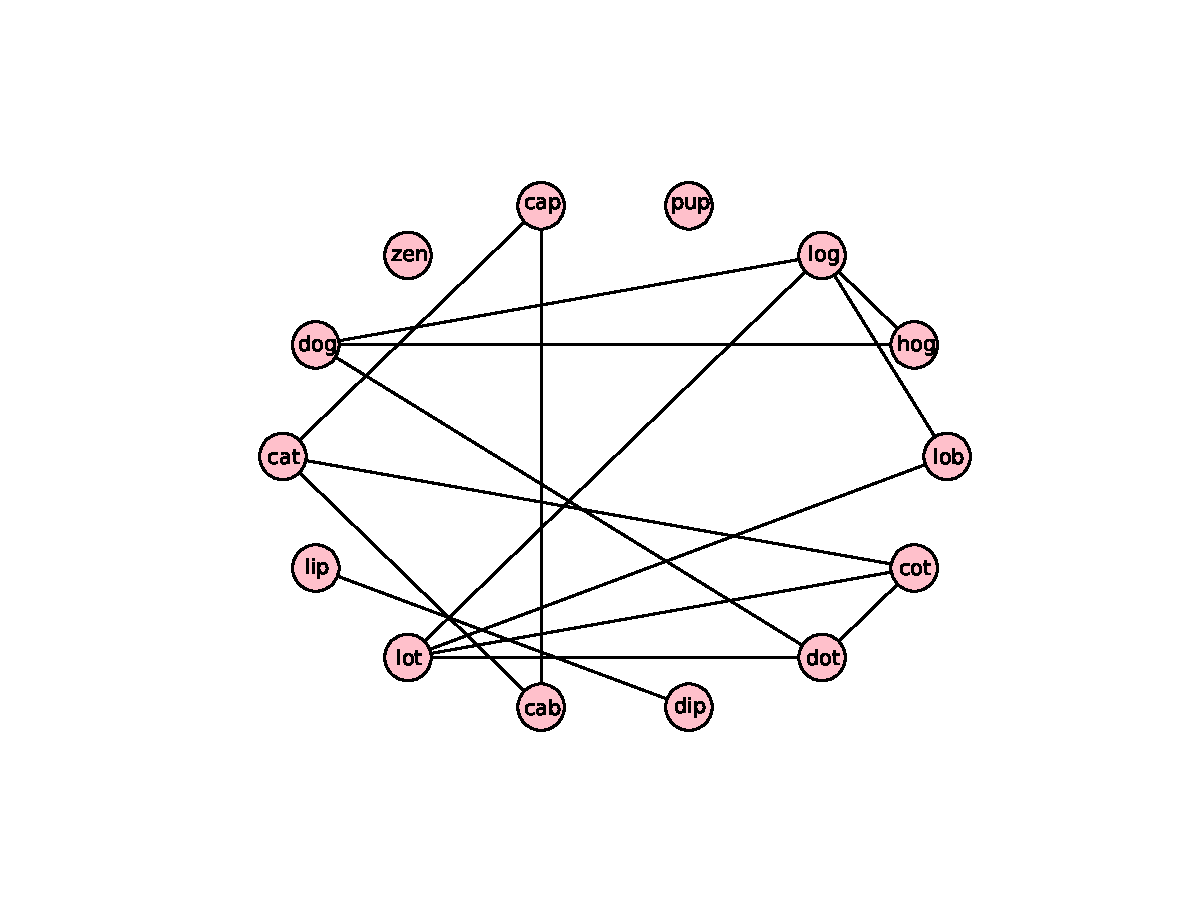
\includegraphics[width=.9\textwidth]{PDFs/toy.pdf}
  \caption{Example phonological network. Each word is a node, and any words that are 1 edit apart are
connected by an edge.}
  \label{fig:toy}
\end{figure}


Figure \ref{fig:networks} shows examples of such networks, where each word is a node, with an edge drawn
between any two words that are phonological neighbors (1 edit away). Words with no or few neighbors are
clustered on the outside. Words with many neighbors are plotted more centrally. As can be seen in Figure
\ref{fig:networks}, substantially more clustering is observed in the more restrictive generative models, but
the real lexicon is, overall, significantly clumpier than the lexicons produced by any of the generative
models.

\begin{figure} \centering
  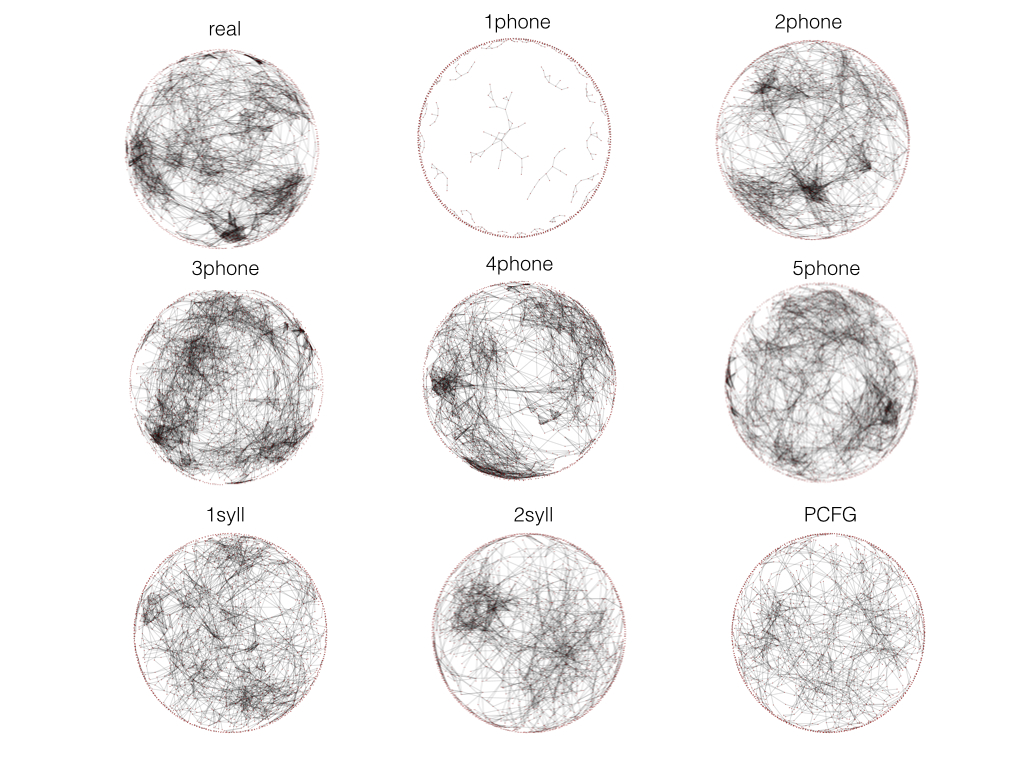
\includegraphics[width=1\textwidth]{networks/net.jpg}
  \caption{Sampling of phonological neighbor network from the different models. Each point is a word, and any
two connected words are phonological neighbors. The simulated lexicons from less constrained generative models
are less clustered and have more isolates (words with no neighbors, plotted on the outside ring).}
  \label{fig:networks}
\end{figure}


\begin{figure}
\centering 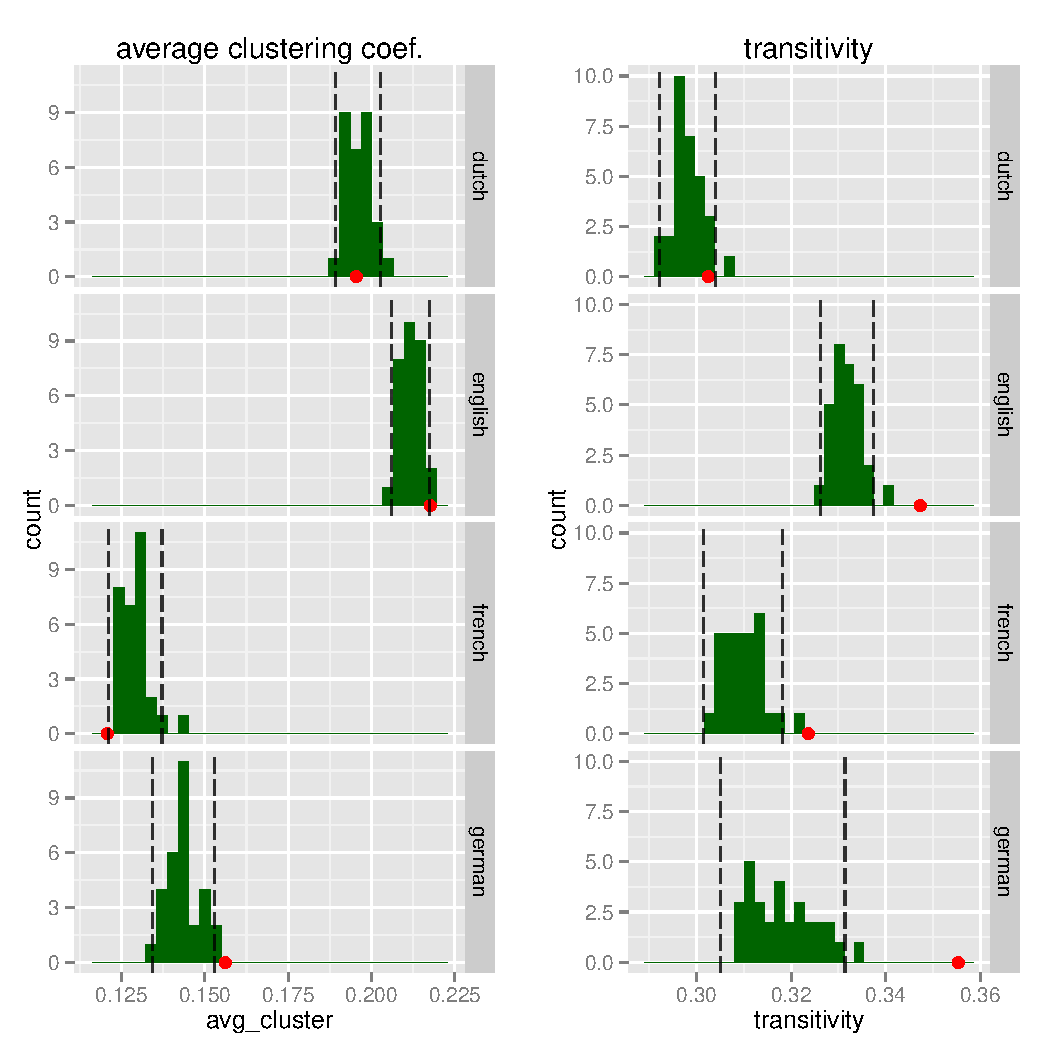
\includegraphics[width=0.8\textwidth]{PDFs/network.pdf}
  \caption{These histograms show the distribution of the most closely matched simulated lexicon (in green)
compared to the real lexicon (the red dot) in terms of network measures for lexical networks (where each node
is a word and any 2 nodes that are minimal pairs are joined in the network): the percent of nodes in the giant
component, the average clustering coefficient, and transitivity. In all cases, the red dot is significantly to
the right of the simulated lexicon distribution--which suggests that the real lexicon is clumpier than
expected by chance. }
  \label{3net}
\end{figure}




\section{Effect of semantics}

As discussed above, there are certain non-trivial effects of semantics in the structure of the lexicon, such
as the presence of semantic clusters like \textit{gl-} words. It is also, of course, the case that certain
words are etymologically related or derived from other words in the lexicon (even when the lexicon is
restricted to morphologically simple words). For example, \textit{skirt} and \textit{shirt} are historically
the Old Norse and Old English form of the same word, whose meanings have since diverged. Both sources of
structure could potentially contribute to pockets of words that are both phonologically and semantically
similar to each other.

To assess whether the presence of these sorts of clusters is driving the clumpiness in the lexicon, we
additionally analyzed the lexicon controlling for semantic factors by defining semantic relatedness scores for
each pair of words in the real lexicon and in the simulated lexicons. Using \cite{fellbaum_wordnet_2010}, we
calculated the \textit{minimum} semantic path distance between any two words of the same primary part of
speech (as defined by CELEX) in the real lexicon\footnote{That is, for any two words in a pair, if their
primary meanings were quite different but their second or third meanings were very similar, the alternate
meanings were used for determining the similarity measure.}. This gives us a semantic relatedness score
between any two words in the real lexicon.

To compare the correlation between semantic relatedness and phonological relatedness in the real lexicon, we
need to compare it to a baseline. One idea would be to randomly permute the semantic relatedness scores from
the real lexicon and arbitrarily assign them to the pairs in the simulated lexicons. But this glosses over an
important source of regularity. It turns out that word pairs that have fewer semantic neighbors systematically
tend to have lower phonotactic probabilities and fewer phonological neighbors. Therefore, word pairs
consisting of low-probability words should also receive lower semantic relatedness scores. Therefore, we
matched each word in the simulated lexicon to a word in the real lexicon by sampling from the appropriate
length, CV, and phonotactic probabiltiy bin. That is, in one lexicon, \textit{jingle} was matched to
\textit{chardle} and \textit{jangle} to \textit{vorset} (orthographic instead of phonetic transcriptions used
for clarity). We assigned the real pair's semantic similarity score to their simulated matched bin. Because
the semantic path distance between \textit{jingle} and \textit{jangle} is 1 (the maximum similarity score),
the 'simulated' semantic distance between \textit{chardle} and \textit{vorset} is also 1.

For each noun in the real lexicon (items listed exclusively as nouns in CELEX), we found its Levenshtein
distance to every other noun. Each of these noun pairs has a matched pair in the simulated lexicon (as with
jingle/jangle and chardle/vorset). We also found the Levenshtein distance for each of the matched pairs in the
simulated lexicon. We can then look at the difference between the real and simulated Levenshtein distance
($RealPairLevenshteinDistance - SimulatedPairLevenshteinDistance$) and the effect of semantic similarity on
phonological similarity.

Specifically, we examined the effect of Wordnet path similarity on Levenshtein distance in a representative
lexicon. Because Wordnet is not reliable for comparing semantic similarity across part of speech categories,
we focused on nouns and restricted the analysis to 4-phone words. Figure \ref{sem_sim} shows the average
difference between the real lexicon Levenshtein distance and the matched pair Levenshtein distance (from a
representative CV and phonotactically matched generative model) on the y-axis. The x-axis is Wordnet semantic
similarity. Closely semantically related words are likely to have a smaller Levenshtein distance than two

One class of words that one might expect should be particularly phonetically distinct is antonyms, like
\textit{hot} and \textit{cold}. Words in such pairs can typically occur in the same linguistic context but
have critically different meanings. In a study of antonyms pairs drawn from Wordnet and restricted to be
mono-morphemic using CELEX, we found that a word is on average more phonetically similar (using Levenshtein
distance) to its antonym than to a random word that is not its antonym. For 43 antonym adjective pairs (86
unique words), the mean Levenshtein distance between a word and its antonym was 3.70 compared to a mean
distance of 4.10 between a word and one of the remaining 84 words ($t = 2.26$, $p < .05$).

\section{Discussion}

We have shown that the English lexicon uses its degrees of freedom in a systematic and interesting way. While
we can still characterize the relationship between word forms and meanings as arbitrary, structure emerges
when one considers the relationships within the space of possible wordforms. The real lexicon is clumpier than
expected by chance, even when controlling for semantic relatedness of words. Across a wide varitey of measures
of phonological confusability and similarity, the real lexicon shows significantly more clustering than even
lexicons produced by the most tightly matched generative model.

Because we focused on mono-morphemic words, the effect cannot be a result of words sharing prefixes and
suffixes. It is also not a product of any structure captured by sound-to-sound transition probabilities or by
a state-of-the-art phonotactic model. Certainly, one explanation for the clumpiness in the lexicon is shared
phonetic properties of semantically related words. Like `skirt' and `shirt', many words in the language share
deep etymological roots. Moreover, the presence of sound symbolism in the lexicon is another source of
structure in the lexicon not captured by our null models. But, since even words that are very distantly
related are more phonetically similar than their matched pair in the simulated lexicon, the lexicon's
clumpiness cannot be attributed only to these factors. Rather, the clumpiness reveals a fundamental drive for
regularity in the English lexicon, a drive that conflicts with the pressure for words to be as phonetically
distinct as possible. This interplay between the competing pressures for sparsity and re-use could underlie
not just the structure of the lexicon discovered here but also the pattern of word learning results shown in
\cite{storkel_differentiating_2006}.

One possible source of the lexicon's clumpiness is that speaker preferentially re-use common articulatory
sequences. That is, beyond just phonotactics and physical constraints, speakers find it easier to articulate
sounds that they already know. Recall our example of the language in which there is only one word for a
speaker to learn. She would quickly become an expert. Along those lines, the presence of any given sound
sequence in the language makes it more likely that the sequence will be re-used in a new word or a new
pronunciation of an existing word. In that sense, the lexicon is ``overfit'': any new word is deeply dependent
on the existing words in the lexicon.

A clumpy lexicon also may allow for easier compression of lexical knowledge. By having words that share many
parts, it may be possible to store words more easily. The fact that more semantically related words are also
more phonetically related supports this hypothesis. It may even be the case that, much as morphology allows
the productive combination of word parts into novel words, there exist sound sequences below the level of the
morpheme that \textit{also} act as productive units of sound.

The interaction of these cognitive and articulatory constraints with the pressure for communicative efficiency
is complex. Despite the fact that one might expect the lexicon to be maximally dispersed for communicative
efficiency, these results strongly suggest that the lexicon is not nearly as sparse as it could be--even given
various phonetic constraints. One possibility is that context is usually enough to disambiguate words, and
therefore it simply does not matter whether certain words are closer together in phonetic space than they
might otherwise be. \cite{piantadosi_communicative_2012} showed that lexical ambiguity, such as the dozens
meanings for short words like \textit{run}, does not impede communication and in fact abets it by allowing the
re-use of short words. In a similar way, there may be a communicative advantage from having not just identical
words re-used but from re-using words that are merely similar. In all cases, context may be enough to
disambiguate the intended meaning and avoid confusion--whether it be confusion between two competing meanings
for the same word or confusion between two similar-sounding words.


More broadly, the methodology used here, whereby the real lexicon is compared to a distribution of
statistically plausible `null' lexicons, could be generalized to answer other questions about the the lexicon
and human language more generally. While much previous work has focused on simply measuring statistical
properties of natural language, modern computing power makes it trivially easy to simulate thousands of
different languages with different constraints, structures, and biases. By comparing real natural language to
a range of simulated possiblities, it is possible to assess what aspects of natural language occur by chance
and which exist for a reason. We hypothesize that other languages will pattern similarly to English, but most
languages lack the tools necessary to adequately calculate phonotactic probability for the analysis presented
here. In future work, we hope to address other languages in order to see whether the clumpiness of the lexicon
varies based on other properties of the language, such as its propensity for borrowing words from other
languages.

In future work, it may be possible to test increasingly sophisticated models of phonotactics using this
methodology. Perhaps our models of phonotactics are simply not good enough yet to capture the rich structure
of natural language. But the results here suggest that any ``null'' model of natural language that can
approximate natural language will need to account for not just the preferred sounds of a language but for the
entire space of existing words. That is, the goodness of ``dax'' as an English word depends not just on an
underlying model of English sound structure but on the fact that ``lax'' is a word, that ``zax'' is not, and
on countless other properties of the existing lexicon.

Indeed, we have shown that the English lexicon is more richly structured than previously thought. The space of
English words is clumpier than any of the null models by a wide variety of measures: minimal pairs both across
and within confusable sets of sounds, network properties, uniqueness of word onsets, and (for shorter words)
edit distance. This property of the lexicon cannot currently be explained by any existing phonotactic models
of English, and we thus conclude that underlying the pressure for sparsity in the lexical system is a deep
drive for regularity and re-use beyond standard levels of lexical and morphological analysis



\bibliographystyle{apacite}


\bibliography{/Users/km/Dropbox/lyx/refs}




\end{document}

